\newpage
\thispagestyle{empty}
% OBS: Coloque sempre o que você quer deixar de fundo na página como primeiro comando

% Imagem de fundo - crie um arquivo separado em tamanho A4 (210x297mm) no formato pdf
\begin{tikzpicture}[remember picture,overlay]
    % Inclui a imagem em segundo plano
    \node[anchor=center,inner sep=0pt] at (current page.center) {
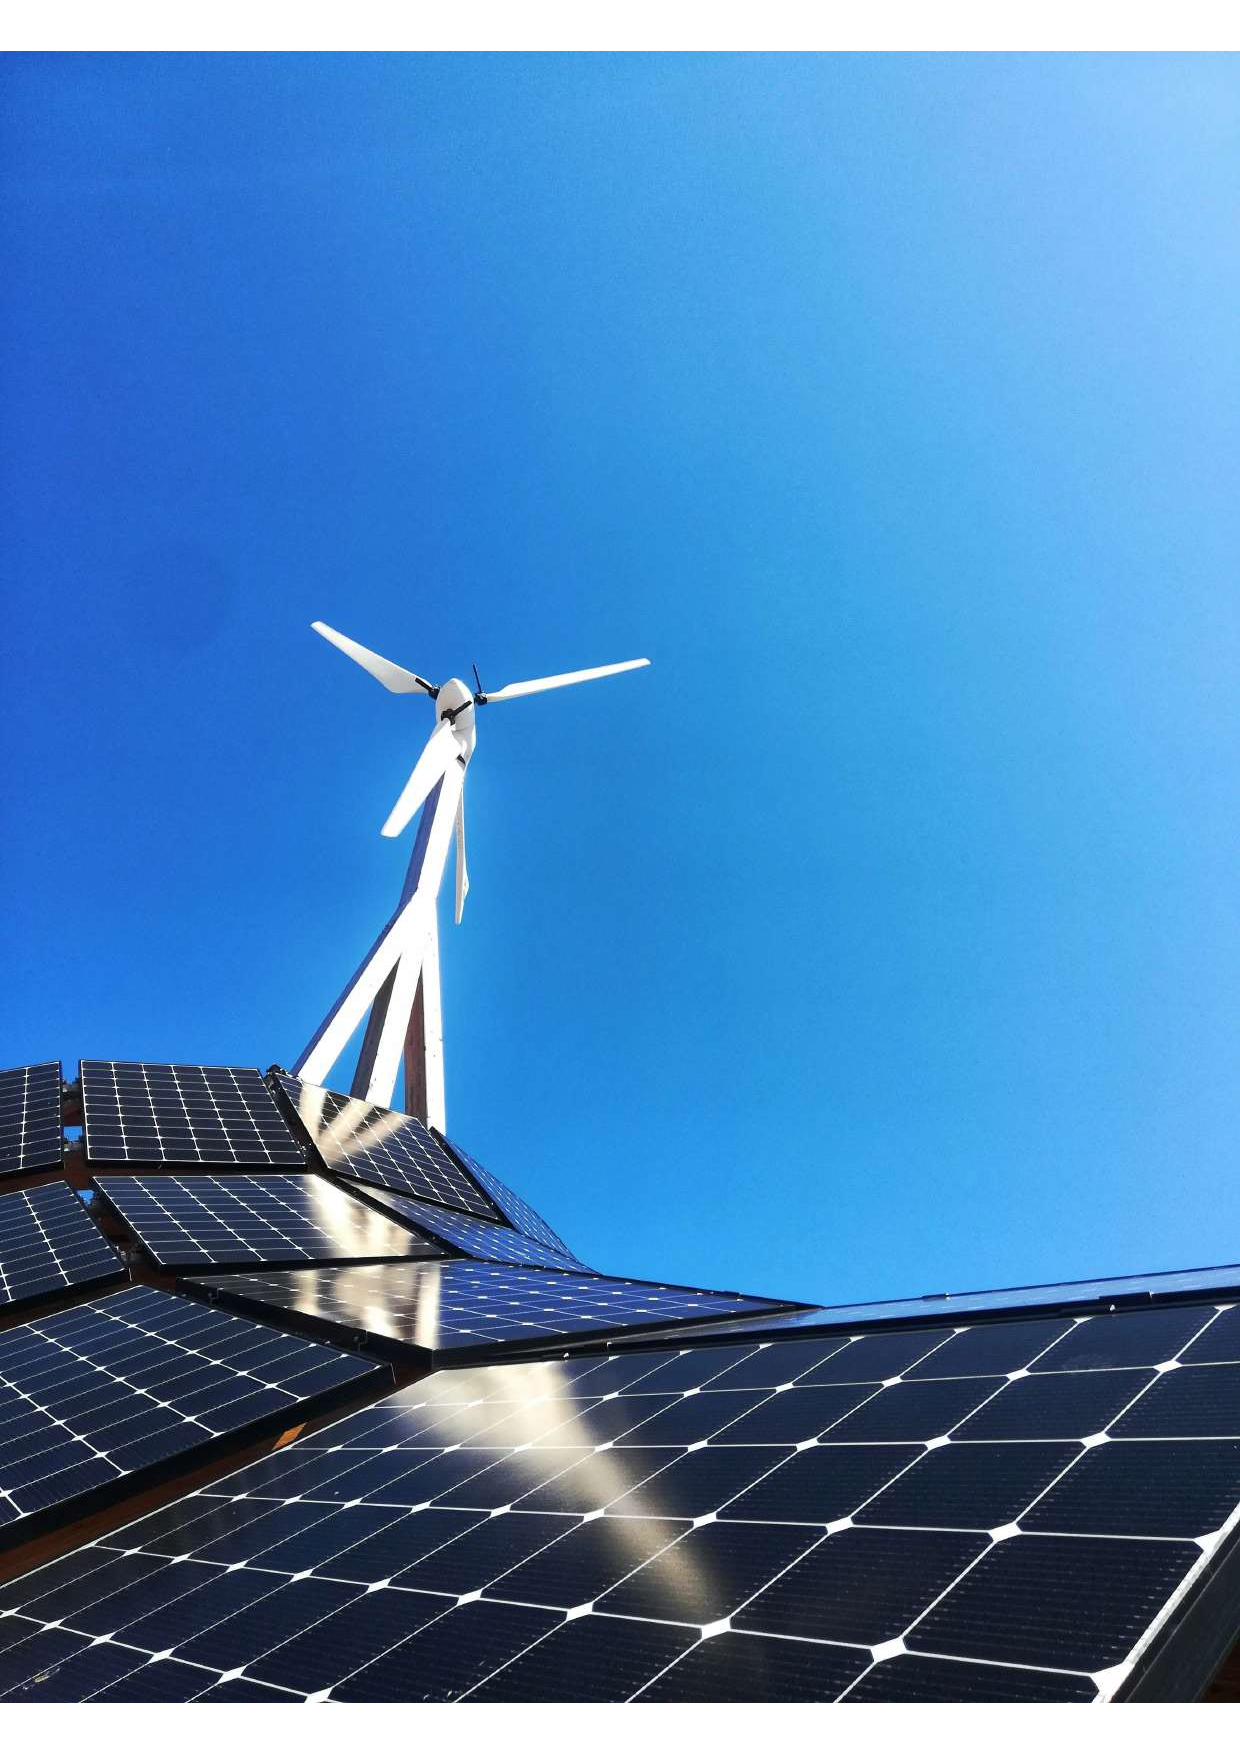
\includegraphics[width=\paperwidth,height=\paperheight,keepaspectratio]{Folha_Rosto/Figs_Folha_Rosto/solar-panel.pdf}
    };
\end{tikzpicture}

% Marcador de página branco
\begin{tikzpicture}[remember picture, overlay, x=1.1pt, y=1.1pt, yscale=-1, xscale=1]
    % Desenho do triângulo com altura aumentada
    \begin{scope}[yshift=-3cm, xshift=-7cm]
        \draw[fill=white, draw=white] 
            (181.51,363.13) -- (181.51,-192.01) -- (390.86,-192.01) -- 
            (390.86,363.13) -- (285.98,431.63) -- (181.56,363.13) -- 
            (181.51,363.13) -- cycle;
    \end{scope}
\end{tikzpicture}

%%LOGO
%% Edite a imagem em um editor gráfico antes de incluí-la no documento LaTex. Ferramentas como GIMP, Inkscape, ou Photoshop podem ser usadas para alterar a cor da imagem (use o arquivo svg da pasta Figs_Folha_Rosto).
%\begin{tikzpicture}[remember picture, overlay]
%  % Adiciona a imagem com um deslocamento usando shift
%  \node at (current page.north west) [anchor=north west, xshift=3.5cm, yshift=-0.9cm] {
%    
\includegraphics[width=6cm]{Folha_Rosto/Figs_Folha_Rosto/divulga-logo.png}
%  };
%\end{tikzpicture}

% NOME DO JORNAL
% Altere a cor e/ou tamanho da fonte no comando \myfontsizeNewstonFolhaRosto e \myfontsizeJornalFolhaRosto  em Structure.tex caso queira outra que não seja a da edição
\begin{tikzpicture}[remember picture, overlay]
  % Adiciona o texto com um deslocamento usando shift
  \node at (current page.north west) [anchor=north west, xshift=3.28cm, yshift=-3.95cm] {
    {\norwester\myfontsizeNewstonFolhaRosto DIVULGA}
  };
   % Adiciona o texto com um deslocamento usando shift
  \node at (current page.north west) [anchor=north west, xshift=3.31cm, yshift=-5.7cm] {
    {\bebasneue\myfontsizeJornalFolhaRosto \textls[530]{AUTOMAÇÃO}}
  };
\end{tikzpicture}


%Número da Edição, coleção (se houver) e data (mês ano)
\begin{tikzpicture}[remember picture, overlay]
  % Desenhar a primeira linha
  \draw[line width=1mm, color=base, shift={(2, -1.5)}] (-1.3,-1) -- (5.4,-1);

  % Adicionar o círculo no meio da linha com um número dentro e preenchido com a cor base
  \node[circle, draw=base, fill=base, minimum size=1cm, inner sep=0pt, text=white, shift={(2, -1.5)}] at (2,-1) {\abrilfatface\myfontsizeEditionFolhaRosto \NumeroEdicao};

  % Adicionar a palavra "Coleção" entre as duas linhas
  \node[shift={(2.1, -2)}, anchor=center] at (0,-1) {\hammersmithone \myfontsizeColecaoData COLEÇÃO \ColecaoEdicao};

  % Adicionar outra palavra ao lado de "Coleção"
  \node[shift={(2, -2)}, anchor=center] at (4,-1) {\hammersmithone \myfontsizeColecaoData \MakeUppercase{\DataEdicao}};

  % Desenhar a segunda linha
  \draw[line width=1mm, color=base, shift={(2, -2.5)}] (-1.3,-1) -- (5.4,-1);

   % Desenhar uma linha pontilhada
   \foreach \i in {0.8, 0.95, 1.10, 1.25, 1.40, 1.55, 1.70, 1.85, 2, 2.15, 2.30, 2.45, 2.60, 2.75, 2.90, 3.05, 3.20} {
  \fill[base, shift={(0, -3.2)}] (\i+2, -1) circle (1pt);
};
  % Tema Principal
  \node[shift={(0, -5)}, anchor=center] at (4, -1) {
    \parbox{5cm}{\centering \hammersmithone \myfontsizeColecaoTema ENERGIAS RENOVÁVEIS:\\[1.5ex]MICRORREDES}
  };
  
  % Desenhar uma linha pontilhada
   \foreach \i in {0.8, 0.95, 1.10, 1.25, 1.40, 1.55, 1.70, 1.85, 2, 2.15, 2.30, 2.45, 2.60, 2.75, 2.90, 3.05, 3.20} {
  \fill[base, shift={(0, -6.9)}] (\i+2, -1) circle (1pt);
};
  % Logo UEM
   \node[shift={(0, -8.5)}, anchor=center] at (4, -1) {
\includegraphics[width=0.1\textwidth]{Figuras_Capa_ContraCapa/ufsc-logo.png}
    };
\end{tikzpicture}


%\begin{tikzpicture}[remember picture, overlay]
%    \node[shift={(4.1, -15)}, anchor=center] at (5.7, -1) {
%        \begin{tikzpicture}
%             % Texto principal com contorno
%            \node[anchor=center, inner sep=0pt, outer sep=0pt] {
%                \parbox{20cm}{\hammersmithone\myfontsizeTituloTema \contour{base}{
%                    \shortstack[l]{DIVULGAÇÃO\\[0.4ex] CIENTÍFICA}}}
%            };
%        \end{tikzpicture}
%    };
%\end{tikzpicture}
\begin{tikzpicture}[remember picture, overlay]
  % Tema Principal
  \node[shift={(4.1, -15)}, anchor=center] at (5.7, -1) {
    \parbox{20cm}{\hammersmithone \myfontsizeDivulgacaoCientifica \textls[150]{
            \contour{base}{\shortstack[l]{DIVULGAÇÃO\\[0.4ex] CIENTÍFICA\\[1ex] E CULTURAL\\[1ex] PARA A\\[1ex] COMUNIDADE}}}}
  };
\end{tikzpicture}



